\documentclass[11pt,a4paper]{jsarticle}

\usepackage[dvipdfmx]{graphicx}
\setlength{\textwidth}{\fullwidth}
\setlength{\textheight}{39\baselineskip}
\addtolength{\textheight}{\topskip}
\setlength{\voffset}{-0.2in}
\setlength{\topmargin}{0pt}
\setlength{\headheight}{0pt}
\setlength{\headsep}{0in}

\title{\Huge{プロジェクトマネジメント演習\\第2班 報告書}}
\author{158576C 新里亮太}
\date{\today}

\begin{document}
\maketitle\thispagestyle{empty}
\newpage
\tableofcontents\thispagestyle{empty}
\newpage

\pagenumbering{arabic}
\setcounter{page}{1}




\section{プロジェクト憲章}
\subsection{プロジェクト名と概要}


本プロジェクトは、「ホログラムで広がる無限の世界」と題し、現在研究・開発が進んでいるホログラム技術と、Fairy Lightsという技術を組み合わせて部屋に投影することで部屋の内装などを変更する。
\subsection{メンバーと組織}
学部生
\begin{itemize}
\item 155702F 大城由也
\item 155708E 中村孝道
\item 155743C 平良柚那
\item 155750F 翁長泰司
\item 155756E 金城愛梨
\item 155757C 平本嶺河
\end{itemize}

院生
\begin{itemize}
\item 158574G 比嘉健太
\item 158576C 新里亮太  
\end{itemize}


\subsection{目標}
部屋の模様替えをする際、かなりのコストと労働力が必要となる。また、宇宙空間や大自然の中で生活することは現代社会に生きる私たちにとって非現実的であると言える。更に、、アレルギーや危険性などで部屋で飼うことのできない動物などもある。これらの問題を解決するために、触ることのできるホログラム技術を用いて部屋の内装を変更したり、動物を投影する。

\subsection{独自性と制約}
独自性
\begin{itemize}
\item プロジェクトメンバーの全員が情報工学科の学生である
\item 触れるホログラムを用いて部屋の内装などを変更する
\item ホログラム投影機を一般家庭に普及させる
\item 現段階では研究中の技術であるFariy Lightsを用いて企画を行う
\end{itemize}

制約
\begin{itemize}
\item 資金がない
\item 講義やアルバイトなどで全員が同じ時間作業できるわけではない
\item 院生を含めたミーティングが週に一度しかない
\item プレゼンテーションに慣れているメンバーが居ない
\end{itemize}

\subsection{成果物}
\begin{itemize}
\item 発表用スライド
\item 最終レポート
\item 予稿
\end{itemize}

\subsection{日程と終了}
\subsubsection{日程}
\begin{itemize}
\item 6月12日 第一回ミーティング
\begin{itemize}
\item ブレーンストーミングによるアイディア出し
\item 成果物報告場所の作成(GoogleDriveにて共有)
\end{itemize}
\item 6月16日 第二回ミーティング
\begin{itemize}
\item テーマ決定
\item ホログラムを用いて何ができるのか話し合い
\end{itemize}
\item 7月3日 第三回ミーティング
\begin{itemize}
\item 中間発表練習
\end{itemize}
\item 7月5日 第四回ミーティング
\begin{itemize}
\item 中間発表練習
\end{itemize}
\item 7月6日 中間発表
\item 7月17日 第五回ミーティング
\begin{itemize}
\item 最終発表の仮原稿添削
\end{itemize}
\item 7月24日 第六回ミーティング
\begin{itemize}
\item 最終レポート添削
\end{itemize}
\item 8月6日 第七回ミーティング
\begin{itemize}
\item 最終発表スライド添削
\end{itemize}
\item 8月7日 第八回ミーティング
\begin{itemize}
\item 最終発表原稿添削
\end{itemize}
\item 8月12日 第九回ミーティング
\begin{itemize}
\item 第一回発表練習
\end{itemize}
\item 8月13日 第十回ミーティング
\begin{itemize}
\item 第二回発表練習
\end{itemize}
\item 8月14日 最終発表
\end{itemize}

\subsubsection{終了}
\begin{itemize}
\item 8月14日のPD最終発表にて発表する。また、スライドや予稿の提出も期限内に行う。
\end{itemize}


\section{プロジェクト計画・実績}
\subsection{目標とスコープ}
\subsubsection{目標}
8月14日のプロジェクトデザイン最終発表にて発表する。また、スライド、予稿を期限内に提出する。
\subsubsection{スコープ}
以下にプロダクトスコープを示す
\begin{itemize}
\item 最終発表スライド
\begin{itemize}
\item 8月14日までにアップロードする
\item 12分の発表に十分収まるスライドを作成する
\end{itemize}
\item 最終レポート
\begin{itemize}
\item 6ページの最終レポートを作成する
\item 企画内容や新規性・社会性など指定された内容を記述する
\end{itemize}
\item 予稿
\begin{itemize}
\item 企画内容やメンバーなどを指定の場所にアップロードする
\item 発表スライドをアップロードする
\end{itemize}
\end{itemize}

\subsection{WBSとアクティビティ}
以下にWBSを示す。


\begin{figure}[htbp]
\begin{center}
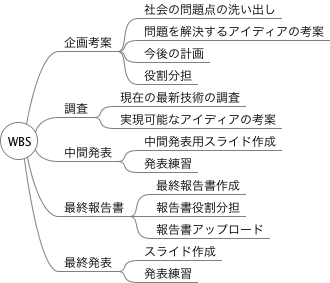
\includegraphics[width=8cm]{WBS.pdf}
\end{center}
\caption{WBS}
\end{figure}

\subsection{スケジュール}
\subsection{リスクと課題}
\subsection{チームとコミュニケーション}
\subsection{実績と品質}
\subsection{応用}
\section{終結}
\subsection{概要}
\subsection{メンバー評価}
\subsection{プロジェクト評価}
\subsection{教訓}
\subsection{講義}
\subsection{関連資料}

\end{document}
